% Appendix A

\chapter{Equetes \& interviews}\label{ch:Enquetes}
\section{Enquetes}\label{sec:enquetes}

Om inzicht te verkrijgen in de belangen van de verschillende stakeholders is een enquete uitgezet naar de interne stakeholders van Eaglescience over SOUP-analyses. De enquete bestond uit 5 vragen en was verzonden naar 15 medewerkers en de response rate was 100\%. Hieronder worden de uikomsten van de enquete besproken.\\

\textbf{Vraag 1: Wat jouw functie binnen Eaglescience?}\\
\begin{figure}[bth]
    \centering
    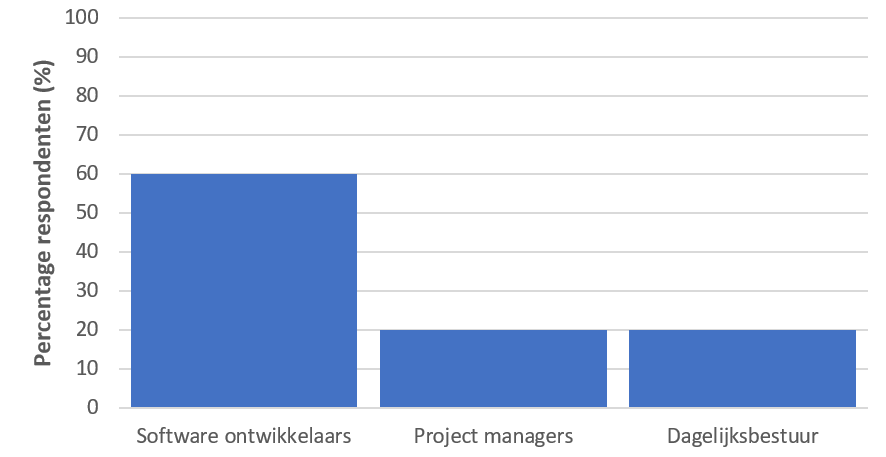
\includegraphics[width=8cm]{gfx/appendix/Vraag1}
    \caption{functies binnen Eaglescience}
    \label{fig:enqueteV1}
\end{figure}

Het leeuwendeel van de respondenten bekleed de functie software ontwikkelaar, terwijl 20\% project managers zijn, en 20\% onder het dagelijks bestuur valt (figuur ~\ref{fig:enqueteV1}).\\

\textbf{Vraag 2: Voer jij zelf SOUP-analyses uit?}\\
\begin{figure}[bth]
    \centering
    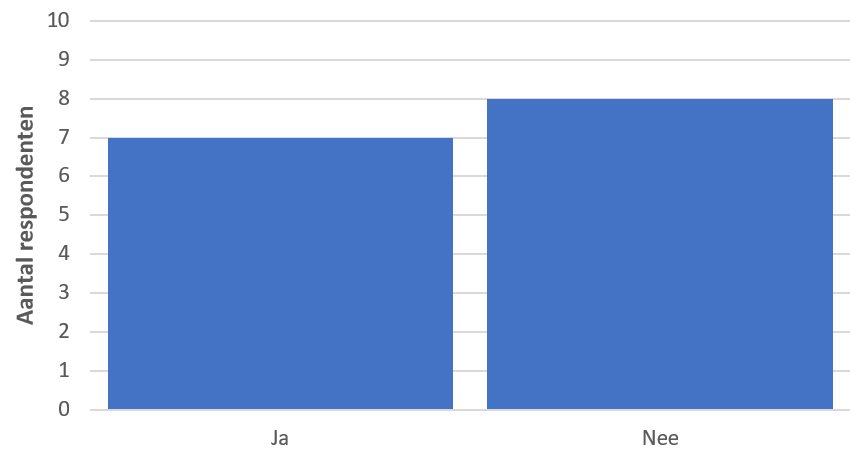
\includegraphics[width=8cm]{gfx/appendix/Vraag2}
    \caption{Voer jij zelf SOUP-analyses uit?}
    \label{fig:enqueteV2}
\end{figure}
Enkel Software ontwikkelaars binnen Eaglescience voeren zelf SOUP-analyses uit, terwijl de overige respondenten dit niet doen. Van de software ontwikkelaars is er een kleine groep die niet zelf betrokken is bij de SOUP-analyses (figuur ~\ref{fig:enqueteV2}).\\

\textbf{Vraag 3: (indien van toepassing) Hoevaak doe je een SOUP-analyse per project en hoeveel tijd schat je hiermee op jaarbasis kwijt te zijn?}\\
\begin{figure}[bth]
    \centering
    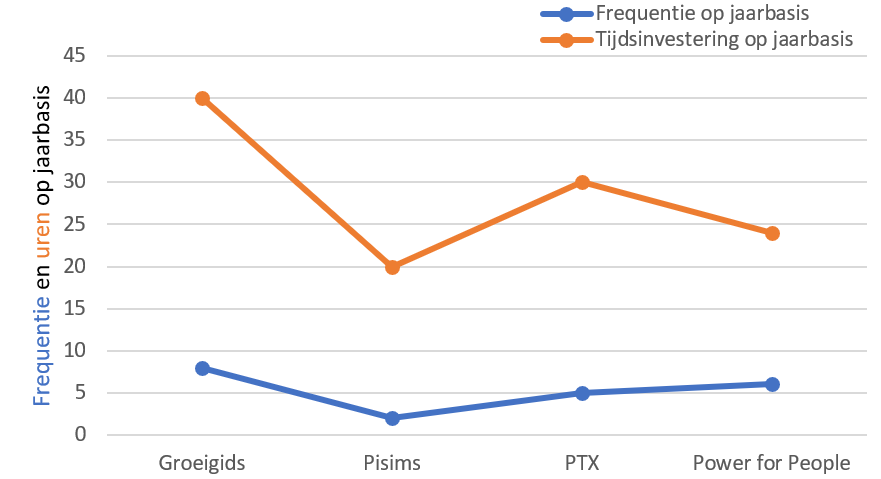
\includegraphics[width=8cm]{gfx/appendix/Vraag3}
    \caption{Hoeveel tijd wordt er besteed aan SOUP-analyses}
    \label{fig:enqueteV3}
\end{figure}

Voor de uitwerking van deze vraag is de totale frequentie en hoeveelheiduren die door de individuele respondenten is ingevuld opgeteld. De grafiek weerspiegeld daarom de totale tijdsinvestering binnen Eaglescience aan SOUP-analyses. Gemiddeld wordt eens per 2 maanden een SOUP-analyse uitgevoerd. De totale werklast op jaarbasis hiervan is $\pm$114 uur (figuur ~\ref{fig:enqueteV3}).\\

\textbf{Vraag 4: Hoe groot acht je het belang van SOUP-analyses?}\\
\begin{figure}[bth]
    \centering
    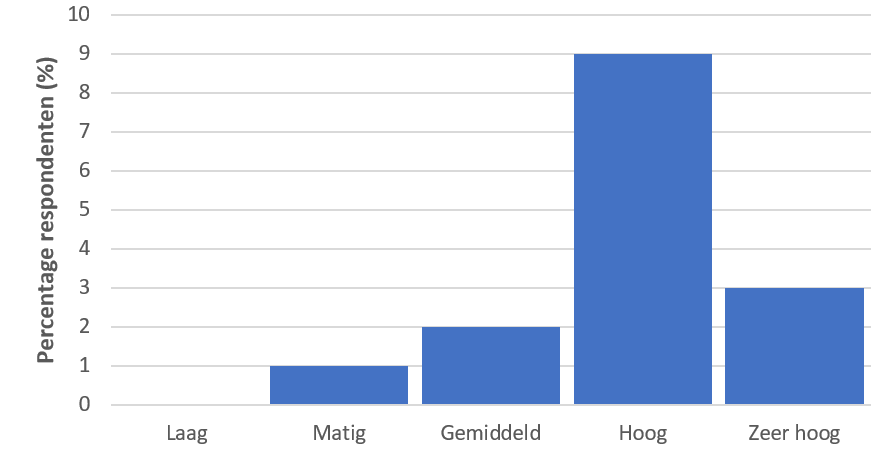
\includegraphics[width=8cm]{gfx/appendix/Vraag4}
    \caption{Het belang van SOUP-analyse}
    \label{fig:enqueteV4}
\end{figure}
Het leeuwendeel van de respondenten gaf aan een groot belang te hechten aan de data verkregen uit SOUP-analyses (figuur ~\ref{fig:enqueteV4}).\\

\textbf{Vraag 5: Worden de uikomsten van SOUP-analyses betrouwbaarder wanneer deze automatische in plaats van handmatig worden uitgevoerd?}\\

\begin{figure}[bth]
    \centering
    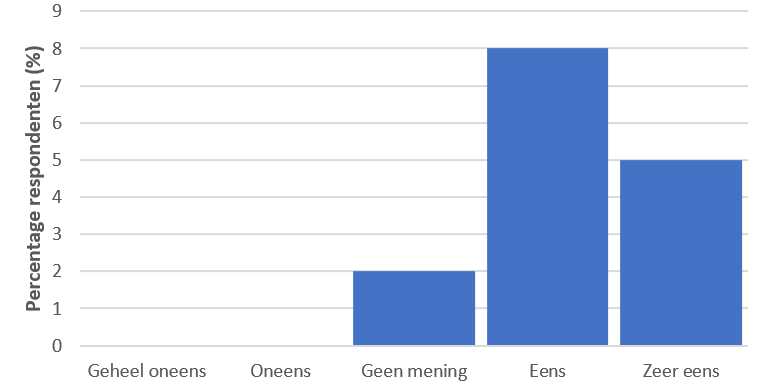
\includegraphics[width=8cm]{gfx/appendix/Vraag5}
    \caption{Betrouwbaarheid van automatisch gegenereerde SOUP-analyse resultaten }
    \label{fig:enqueteV5}
\end{figure}

De repondenten waren het bijna unaniem eens dat het automatisch uitvoeren van SOUP analyses betrouwbaardere resultaten geeft dan wanneer dit handmatig wordt gedaan (figuur ~\ref{fig:enqueteV5}).

\clearpage
\section{Interviews}\label{sec:interviews}

\subsection{Ontwikkelaar}\label{subsec:ontwikkelaar}
Dit gesprek heeft als \textbf{doel} om te achterhalen welke taken er op dit moment worden uitgevoerd op het gebied van SOUP-analyses en hoeveel tijd hierin wordt geinvesteerd. Daarnaast is er gevraagd welke verbeteringen er vanuit zijn rol zijn. Dit gesprek heeft plaatsgevonden op 20-20-2020 met [NAAM].\smallskip

\textbf{Introductie }
Aangegeven dat het gesprek vertrouwelijk is, en dat de tekst hierover ge-edit mag worden door de geinterviewde, als ook welke functie er bekleed wordt door de geinterviewde. De volgende vragen zijn tijdens het interview gesteld:
\\
\textbf{Welke stappen worden er op dit moment genomen om er zo zeker mogelijk van te zijn dat er geen kwetsbaarheden zitten in de code? }
\\

\textbf{Heb je het idee dat de tijd die nodig is om deze stappen te zetten opweegt tegen het behaalde resultaat?}
\\

\textbf{Is het resultaat van het werk zichtbaar voor iedereen?}
\\

\textbf{Wat zou volgens jou een ideale situatie zijn mocht je een module mogen ontwikkelen om de SOUP-analyse automartisch te doen?  }
\\

\textbf{Heb je aanvullingen of opmerkingen op basis van de eerder naar je toegestuurde requirements?}
\\



%
%
%In deze appendix zijn de verslagen te vinden van de verschillende interviews die gehouden zijn met de verschillende betrokkenen. Bij alle gesprekken die gevoerd zijn is aangegeven dat alles wat er tijdens de gesprekken besproken wordt desgewenst anoniem verwerkt wordt en dat het verslag na te lezen is voordat er iemand anders naar gekeken heeft.
%\section{Interviews met betrokkenen van de nieuwe module voor SOUP analyse}\label{sec:intake-gesprek-oprachtgever}
%Deze interviews zijn gehouden met geselecteerde personen die vanuit hun functie direct betrokken zijn met SOUP analyses. Het \textbf{doel} van deze interviews in het deels het achterhalen van de huidige manier van het doen van een SOUP-analyse. En deels hun visie op mogelijke verbeteringen die de nieuwe methode zou kunnen bieden.
%
%\subsection{Ontwikkelaar}\label{subsec:ontwikkelaar}
%Dit gesprek heeft als \textbf{doel} om te achterhalen welke taken er op dit moment worden uitgevoerd op het gebied van SOUP-analyses. Als ook de tijd die het kost. Daarnaast is er gevraagd welke verbeteringen er vanuit zijn rol zijn. Dit gesprek heeft plaatsgevonden op 20-20-2020 met [NAAM].\smallskip
%
%\textbf{Introductie }
%Aangegeven dat het gesprek vertrouwelijk is in de zin dat het geeddit mag worden door de geinterviewde, als ook welke functie er bekleed wordt door de geinterviewde.
%\\
%\textbf{Welke stappen worden er op dit moment genomen om er zo zeker mogelijk van te zijn dat we geen kwetsbaarheden hebben in onze code? }
%\\
%\textbf{Heb je het idee dat de tijd die nodig is om deze stappen te zetten opweegt tegen het resultaat?}
%\\
%\textbf{Is het resultaat van het werk zichtbaar voor iedereen?}
%\\
%\textbf{Wat zou volgens jou een ideale situatie zijn mocht je een module mogen ontwikkelen om de SOUP-analyse automartisch te doen?  }
%\\
%\textbf{Op basis van de getoonde requirements tot nu toe zijn er aanvullingen die direct tot je komen?}
%\\
%\subsection{Project manager}\label{subsec:project-manager}
%Dit gesprek heeft als \textbf{doel} de informatie behoeften van een projectmanager in kaart te brengen. Dit gesprek heeft plaatsgevonden op 20-20-2020 met [NAAM]
%\\
%\textbf{Introductie }
%Aangegeven dat het gesprek vertrouwelijk is in de zin dat het geeddit mag worden door de geinterviewde, als ook welke functie er bekleed wordt door de geinterviewde.
%\\
%\textbf{Hoe verkrijg je op dit moment de informatie om beslissingen te nemen om kwetsbaarheden op te lossen? }
%\textbf{Zou het volgens jou verschil uitmaken dat er automatisch een analyse wordt uitgevoerd ten opzichte van de kwaliteit van de software?}
%\\
%\textbf{Zou dit dan ook ten goede komen met betrekking tot budgetten en dergelijke. Met andere woorden zouden ontwikkelaars meer tijd hebben om te ontwikkelen?}
%\\
%\textbf{Op welke manieren zou je de informatie willen zien in de portal, is het handig om te weten wanneer een scan is uitgevoerd?}
%\\
%\textbf{Op basis van de getoonde requirements tot nu toe zijn er aanvullingen die direct tot je komen?}
%
%\subsection{Managment teamlid}\label{subsec:managment-teamlid}
%Dit gesprek heeft als \textbf{doel} om te achterhalen welke voordelen het managment team ziet in de nieuwe methode en module. Dit gesprek heeft plaats gevonden op 20-20-2020 met [NAAM]
%\\
%\textbf{Introductie }
%Aangegeven dat het gesprek vertrouwelijk is in de zin dat het geeddit mag worden door de geinterviewde, als ook welke functie er bekleed wordt door de geinterviewde.
%\\
%\textbf{Naast efficiëntie welke andere voordelen zie je met de implementatie van de nieuwe module?}
%\\
%\textbf{Op welke manieren zou je de informatie willen zien in de portal, is het handig om te weten wanneer een scan is uitgevoerd?
%\\
%\textbf{Op basis van de getoonde requirements tot nu to zijn er aanvullingen die direct tot je komen?}
%\\
%
%
%
%\section{Interviews met collega's over de dev-stack die gebruikt wordt binnen EagleScience}\label{sec:dev-stackInterviews}
%
%Het \textbf{doel} van deze gesprekken is inzicht krijgen in de reden waarom we bepaalde tools en ontwikkeltalen gebruiken binnen EagleScience. Bij alle gesprekken die gevoerd zijn is er aangegeven dat het verslag nagekeken mag worden. Er geanonimiseerd mag worden. Ook heb ik aangegeven waar nodig dat ik het gesprek opneem en alleen gebruik als input voor het onderzoek en de implementatie. Daarnaast heb ik er voor gekozen om semigestructureerde gesprekken te voeren waarin vooraf een doel heb verkondigd. De reden voor de beslissing is dat door de manier waarop EagleScience voor haar klanten werkt er niet veel tijd overblijft voor niet inplanbare uren.
%
%\subsection{Gesprek over Scala met Bas Broere}\label{subsec:gesprek-over-scala-met-bas-broere}
%Het \textbf{doel} van dit gesprek is om er achter te komen hoe en waarom we Scala gebruiken. Een aantal
%\textbf{Introductie: }\\
%Inleiding gegeven over het doel van het gesprek en dat het verslag nakeken mag worden en dat desgewenst delen kunnen worden geanonimiseert
%\subsection{}\label{subsec:dev-stackVragen}
%
